\documentclass[aspectratio=43]{beamer}

%\usetheme{Singapore}
\usetheme[hideallsubsections]{Madrid}
\usecolortheme{beaver}
\usefonttheme{structurebold}
\useinnertheme{circles}
\useoutertheme[[footline=authortitle, subsection=false]{miniframes}


\setbeamersize{text margin left=5mm, text margin right=5mm} % bit more white space at sides


\usepackage{graphicx}
\graphicspath{{graphics/}}

\usepackage{animate}
\usepackage{tikz}
\usetikzlibrary{calc, positioning, matrix, fit, backgrounds, chains}
\usepackage{pgfpages}
\usepackage[normalem]{ulem}

% magic to allow tikz nodes to use onslide
\tikzset{onslide/.code args={<#1>#2}{%
  \only<#1>{\pgfkeysalso{#2}} % \pgfkeysalso doesn't change the path
}}


% suppress navigation symbols
\setbeamertemplate{navigation symbols}{}

% Some colours
\colorlet{notgreen}{blue!50!yellow}

\title{Linear models}
% \author{Samraat Pawar }
%\institute{Imperial College London}
\date{}


\begin{document}

% hide navigation sections for first slides
%\setbeamertemplate{miniframes}{}

% turn off shrinking sub items in nested lists
\setbeamerfont{itemize/enumerate subbody}{size=\normalsize}
\setbeamerfont{itemize/enumerate subsubbody}{size=\normalsize}

%%%%%%%%%%%%%%%%%%%%%%%%%%%%%%%%%%%%%%%%%%%%%%%%%%%%%%%%%%%%%%%%%%%%%
\frame{\titlepage}

\frame
{
  \frametitle{Course aims}

  \begin{itemize}
  \item Learn a core set of statistical skills 
  \item Practice using a professional statistical program
  \item Develop ability to build, criticise and interpret linear models
  \end{itemize}
  \vspace{12pt}
  The aim of this lecture:
  \begin{itemize}
  \item Underpinning theory of linear models
  \item Introduce concepts to be developed using practicals
  \end{itemize}
}

% \frame{
  % \frametitle{Aim for today}

% \centering
% 
\includegraphics[height=0.8\textheight]{dontpanic-marvin-ltr.jpeg}

% }


%%%%%%%%%%%%%%%%%%%%%%%%%%%%%%%%%%%%%%%%%%%%%%%%%%%%%%%%%%%%%%%%%%%%%
\frame
{
  \frametitle{Lecture structure}



  \begin{itemize}
  \item What is a linear model?
  \item How do we deal with variation?  
  \item Is a linear model appropriate for the data?
  \item How well does a linear model explain the data?
  \end{itemize}

  \vspace{12pt}
  Concepts:
  \begin{itemize}
  \item Types of variable: continuous versus categorical 
  \item Terms and coefficients of a model
  \item Model residuals
  \item Significance testing
  \end{itemize}

}

\section{What is a linear model?}


%%%%%%%%%%%%%%%%%%%%%%%%%%%%%%%%%%%%%%%%%%%%%%%%%%%%%%%%%%%%%%%%%%%%%
\frame
{\frametitle{What predicts the weights ($w$) of lecturers?}



Use our {\it hypotheses} to identify the {\it variables} we collect\ldots
\begin{itemize}

	\item Height ($h$) in metres
	\item Exercise per week ($e$) in hours
	\item Gender ($g$)
	\item Distance from home to nearest Greggs bakery ($d$) in metres
	\item Ownership of a games console ($c$)

\end{itemize}
\vspace{12pt}
\ldots and build a mathematical model:
\[w = \beta_1 + \beta_2 h + \beta_3 e + \beta_4 g_m  + \beta_5 d + \beta_6 c_s + \beta_7 c_a + \varepsilon\]
}

%%%%%%%%%%%%%%%%%%%%%%%%%%%%%%%%%%%%%%%%%%%%%%%%%%%%%%%%%%%%%%%%%%%%%
\begin{frame}[t]
\frametitle{A combination of four components}

\begin{center}

%% Fix the equation in place on the slide 
%% - avoid absolute tikz positions because the overlay makes it hard to 
%%   get the rest of the slide aligning correctly.
%% - using a bounding box forces the underlying text down to the same level
\begin{tikzpicture} 

\useasboundingbox (0 mm, 0mm) rectangle (118 mm, 30mm); % width of slide less margins - fixed (128 - 2 x 5)

% style fix minimum height on nodes to align labels above components, 
% a chain to align the equation along and some colour styles for overlays
\begin{scope}[every node/.style={text height=3mm,  text depth=1mm, on chain, inner sep=0.5mm},
              gr/.style={teal}, 
              rd/.style={red}, 
              bl/.style={blue}, 
              gy/.style={gray},
              start chain, node distance=0mm]

\node [gr] (w) at (12mm, 19mm) {$w$}; % fixed position within bbox
\node      (eq) {$=$};
\node [rd] (b1) {$\beta_1$};
\node      (p)  {$+$};
\node [rd] (b2) {$\beta_2$};
\node [bl] (h)  {$h$};
\node      (p)  {$+$};
\node [rd] (b3) {$\beta_3$};
\node [bl] (e)  {$e$};
\node      (p)  {$+$};
\node [rd] (b4) {$\beta_4$};
\node [bl] (g)  {$g_m$};
\node      (p)  {$+$};
\node [rd] (b5) {$\beta_5$};
\node [bl] (d)  {$d$};
\node      (p)  {$+$};
\node [rd] (b6) {$\beta_6$};
\node [bl] (cS)  {$c_s$};
\node      (p)  {$+$};
\node [rd] (b7) {$\beta_7$};
\node [bl] (cA)  {$c_a$};
\node      (p)  {$+$};
\node [gy] (eps)  {$\varepsilon$};


\end{scope}

\begin{scope}[every node/.style={rounded corners, draw, minimum height=6mm},
              every path/.style={latex-, draw=red, thick}]
              
    \node (exp)  [inner sep=0pt, yshift=1cm, fit={(e) (cS)}, label=center:Explanatory variables, fill=blue!10, draw=blue] {};	
    \node (coef) [inner sep=0pt, yshift=-1cm, fit={(b2) (b6)}, label=center:Coefficients, fill=red!10, draw=red] {};	
	\node (resp)  [above = 4mm of w, fill=teal!10, draw=teal] {Response variable};
	\node (resid)  [below = 4.5mm of eps, fill=gray!10, draw=gray] {Residuals};

	\foreach \i in {e, d, g, cS}  \draw [blue] (\i.north) -- (\i.north |- exp.south);
	\draw [blue] (cA.north) |- (exp.east);
	\draw [blue] (h.north) |- (exp.west);	
	\foreach \i in {b2, b3, b4, b5, b6}  \draw [red] (\i.south) -- (\i.south |- coef.north);
	\draw [red] (b7.south) |- (coef.east);
	\draw [red] (b1.south) |- (coef.west);
    \draw [teal] (w.north) --  (resp.south);
    \draw [gray] (eps.south) -- (resid.north);

    
\end{scope}

\end{tikzpicture}


\begin{itemize}
\item A \textcolor{teal}{response variable} ($w$)
\item A set of \textcolor{blue}{explanatory variables} ($h,e,g,d,c$)
\item A set of \textcolor{red}{coefficients} ($\beta_1$ -- $\beta_7$)
\item A set of \textcolor{gray}{residuals} ($\varepsilon$)
\end{itemize}

\end{center}
\end{frame}

%%%%%%%%%%%%%%%%%%%%%%%%%%%%%%%%%%%%%%%%%%%%%%%%%%%%%%%%%%%%%%%%%%%%%
\begin{frame}[t]
\frametitle{Different types of variables}

\begin{center}
\begin{tikzpicture} 

\useasboundingbox (0 mm, 0mm) rectangle (118 mm, 30mm); % width of slide less margins - fixed (128 - 2 x 5)

% style fix minimum height on nodes to align labels above components, 
% a chain to align the equation along and some colour styles for overlays
\begin{scope}[every node/.style={text height=3mm,  text depth=1mm, on chain, inner sep=0.5mm},
              gr/.style={teal}, 
              rd/.style={red}, 
              bl/.style={blue}, 
              gy/.style={gray},
              start chain, node distance=0mm]

\node [bl] (w) at (12mm, 19mm) {$w$}; % fixed position within bbox
\node      (eq) {$=$};
\node [gy] (b1) {$\beta_1$};
\node      (p)  {$+$};
\node [gy] (b2) {$\beta_2$};
\node [bl] (h)  {$h$};
\node      (p)  {$+$};
\node [gy] (b3) {$\beta_3$};
\node [bl] (e)  {$e$};
\node      (p)  {$+$};
\node [gy] (b4) {$\beta_4$};
\node [rd] (g)  {$g_m$};
\node      (p)  {$+$};
\node [gy] (b5) {$\beta_5$};
\node [bl] (d)  {$d$};
\node      (p)  {$+$};
\node [gy] (b6) {$\beta_6$};
\node [rd] (cS)  {$c_s$};
\node      (p)  {$+$};
\node [gy] (b7) {$\beta_7$};
\node [rd] (cA)  {$c_a$};
\node [gy] (p)  {$+$};
\node [gy] (eps)  {$\varepsilon$};


\end{scope}

\begin{scope}[every node/.style={rounded corners, draw, minimum height=6mm},
              every path/.style={latex-, draw=red, thick}]
              
    \node (cont)  [inner sep=0pt, yshift=1cm, fit={(w) (d)}, label=center:Continuous variables, fill=blue!10, draw=blue] {};	
    \node (cat) [inner sep=0pt, yshift=-1cm, fit={(g) (cA)}, label=center:Categorical variables, fill=red!10, draw=red] {};	

	\foreach \i in {w, h, e, d}  \draw [blue] (\i.north) -- (\i.north |- exp.south);   
	\foreach \i in {g, cA, cS}  \draw [red] (\i.south) -- (\i.south |- coef.north);   
    
\end{scope}

\end{tikzpicture}

\begin{itemize}
\item The response variable is always \textcolor{blue}{continuous}.
\item The explanatory variables can be a mix of:
\begin{itemize}
\item \textcolor{blue}{Continuous} variables: height, exercise and distance.
\item \textcolor{red}{Categorical} variables: gender and console ownership.
\end{itemize}
\item \textcolor{red}{Categorical} variables or {\it factors} have a number of {\it levels}:
\begin{itemize}
\item Gender has two levels (Male / Female)
\item Console has three levels (None / Sofa-based / Active)
\end{itemize}
\end{itemize}
\end{center}
\end{frame}


\begin{frame}[t]
\frametitle{Terms and coefficients}

\begin{center}
\begin{tikzpicture} 

\useasboundingbox (0 mm, 0mm) rectangle (118 mm, 30mm); % width of slide less margins - fixed (128 - 2 x 5)

% style fix minimum height on nodes to align labels above components, 
% a chain to align the equation along and some colour styles for overlays
\begin{scope}[every node/.style={text height=3mm,  text depth=1mm, on chain, inner sep=0.5mm},
              gr/.style={teal}, 
              rd/.style={red}, 
              bl/.style={blue}, 
              gy/.style={gray},
              start chain, node distance=0mm]

\node [bl] (w) at (12mm, 19mm) {$w$}; % fixed position within bbox
\node      (eq) {$=$};
\node [gy] (b1) {$\beta_1$};
\node      (p)  {$+$};
\node [gy] (b2) {$\beta_2$};
\node [bl] (h)  {$h$};
\node      (p)  {$+$};
\node [gy] (b3) {$\beta_3$};
\node [bl] (e)  {$e$};
\node      (p)  {$+$};
\node [gy] (b4) {$\beta_4$};
\node [rd] (g)  {$g_m$};
\node      (p)  {$+$};
\node [gy] (b5) {$\beta_5$};
\node [bl] (d)  {$d$};
\node      (p)  {$+$};
\node [gy] (b6) {$\beta_6$};
\node [rd] (cS)  {$c_s$};
\node      (p)  {$+$};
\node [gy] (b7) {$\beta_7$};
\node [rd] (cA)  {$c_a$};
\node [gy] (p)  {$+$};
\node [gy] (eps)  {$\varepsilon$};


\end{scope}

\begin{scope}[every node/.style={rounded corners, draw, minimum height=6mm},
              every path/.style={latex-, draw=red, thick}]
              
    \node (height)    [below=0.5cm of h, fill=blue!10, draw=blue, xshift=-3mm] {Height};
    \draw [blue] (h.south) -- (h.south |- height.north);

    \node (exercise)  [below=0.5cm of e, fill=blue!10, draw=blue, xshift=4mm] {Exercise};
    \draw [blue] (e.south) -- (e.south |- exercise.north);

    \node (distance)  [below=0.5cm of d, fill=blue!10, draw=blue] {Distance};
    \draw [blue] (d.south) -- (d.south |- distance.north);

    \node (gender)  [above=0.5cm of g, fill=red!10, draw=red] {Gender};
    \draw [red] (g.north) -- (g.north |- gender.south);

    \node (console) [inner sep=0pt, yshift=1.1cm, fit={(cA) (cS)}, label=center:Console, fill=red!10, draw=red] {};	
    \foreach \i in {cA, cS}  \draw [red] (\i.north) -- (\i.north |- console.south);   
    
\end{scope}

\end{tikzpicture}


\begin{itemize}
\item Each explanatory variable is a {\it term} in the model
\item Each term has at least one coefficient
\item \textcolor{blue}{Continuous} terms always have one coefficient
\item \textcolor{red}{Factors} have $N - 1$ coefficients, where $N$ is the number of levels

\end{itemize}
\end{center}
\end{frame}



%:

\begin{frame}[t]
\frametitle{Wait! Why $N-1$? What is $\beta_1$?}

\begin{center}
\begin{tikzpicture}[every node/.style={text height=3mm,  text depth=1mm, on chain, inner sep=0.5mm},
              gr/.style={teal}, 
              rd/.style={red}, 
              bl/.style={blue}, 
              gy/.style={gray},
              pr/.style={draw, rounded corners=2mm, gray},
              start chain, node distance=0mm]

\useasboundingbox (0 mm, 0mm) rectangle (118 mm, 21mm); % width of slide less margins - fixed (128 - 2 x 5)

\node  (w) at (12mm, 10mm) {$w$}; % fixed position within bbox
\node  (eq) {$=$};
\node  (b1) {$\beta_1$};
\node  (p)  {$+$};
\node  (b2) {$\beta_2$};
\node  (h)  {$h$};
\node  (p)  {$+$};
\node  (b3) {$\beta_3$};
\node  (e)  {$e$};
\node  (p)  {$+$};
\node  (b4) {$\beta_4$};
\node  (g)  {$g_m$};
\node  (p)  {$+$};
\node  (b5) {$\beta_5$};
\node  (d)  {$d$};
\node  (p)  {$+$};
\node  (b6) {$\beta_6$};
\node  (cS)  {$c_s$};
\node  (p)  {$+$};
\node  (b7) {$\beta_7$};
\node  (cA)  {$c_a$};
\node  (p)  {$+$};
\node  (eps)  {$\varepsilon$};

\node [pr, red, fit= (b1), line width=1pt] {};
\node [pr, fit= (b2) (h)] {};
\node [pr, fit= (b3) (e)] {};
\node [pr, fit= (b4) (g)] {};
\node [pr, fit= (b5) (d)] {};
\node [pr, fit= (b6) (cS)] {};
\node [pr, fit= (b7) (cA)] {};

\end{tikzpicture}
%

\begin{itemize}
\item Two ways of thinking about $\beta_1$:
\begin{itemize}
\item Continuous variables: the $y$ {\it intercept}
\item Factors: the baseline or {\it reference} value
\end{itemize}
\item This baseline is the value for the {\it first levels} of each factor
\item All response values start at this baseline
\item All the other coefficients measure {\it differences} from $\beta_1$:
\begin{itemize}
\item along a continuous slope
\item as an offset to a different level
\end{itemize}
\end{itemize}

\end{center}

\end{frame}

\begin{frame}[t]
\frametitle{Linear models are just a sum}

\begin{center}
\begin{tikzpicture}[every node/.style={text height=3mm,  text depth=1mm, on chain, inner sep=0.5mm},
              cross/.style={path picture={
                   \draw[red, ultra thick] (path picture bounding box.center) +(0, 1.4mm) -- +(0, -1.4mm) (path picture bounding box.center) +(1.4mm, 0mm) -- +(-1.4mm,0) ;}},
              gr/.style={teal}, 
              rd/.style={cross, red}, 
              bl/.style={blue}, 
              gy/.style={gray},
              pr/.style={draw, rounded corners=2mm, gray},
              start chain, node distance=0mm]

\useasboundingbox (0 mm, 0mm) rectangle (118 mm, 21mm); % width of slide less margins - fixed (128 - 2 x 5)

\node      (w) at (12mm, 10mm) {$w$}; % fixed position within bbox
\node      (eq) {$=$};
\node      (b1) {$\beta_1$};
\node [rd] (p)  {$+$};
\node      (b2) {$\beta_2$};
\node      (h)  {$h$};
\node [rd] (p)  {$+$};
\node      (b3) {$\beta_3$};
\node      (e)  {$e$};
\node [rd] (p)  {$+$};
\node      (b4) {$\beta_4$};
\node      (g)  {$g_m$};
\node [rd] (p)  {$+$};
\node      (b5) {$\beta_5$};
\node      (d)  {$d$};
\node [rd] (p)  {$+$};
\node      (b6) {$\beta_6$};
\node      (cS)  {$c_s$};
\node [rd] (p)  {$+$};
\node      (b7) {$\beta_7$};
\node      (cA)  {$c_a$};
\node [rd] (p)  {$+$};
\node      (eps)  {$\varepsilon$};

\end{tikzpicture}
%
\end{center}

\begin{itemize}
\item Find the baseline value for women with no games console ($\beta_1$)
\item The model tells us how much to add to this\ldots
\begin{itemize}
\item  for a height of 1.82 metres?
\item  for doing 150 minutes of exercise a week?
\item  for being male?
\item  for living 2416 metres from a Greggs?
\item  for owning an Xbox?
\end{itemize}
\end{itemize}


\end{frame}


\frame
{\frametitle{Examples - one continuous variable}

\begin{columns}[T]

	\column{0.5\textwidth}
		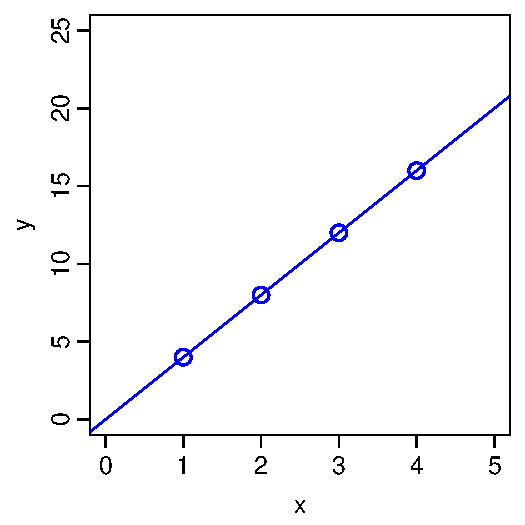
\includegraphics[width=\textwidth]{Origin.pdf}
		
	\column{0.5\textwidth}
		\begin{align*}
		  y  &=  \beta_1 x \\
		  \\
		  4  &=  4 \times 1 \\
		  8  &=  4 \times 2 \\
		  12 &=  4 \times 3 \\
		  16 &=  4 \times 4   
		\end{align*}
		\[\beta_1 =4\]
\end{columns}
}


\frame
{\frametitle{Examples - one continuous variable}

\begin{columns}[T]

	\column{0.5\textwidth}
		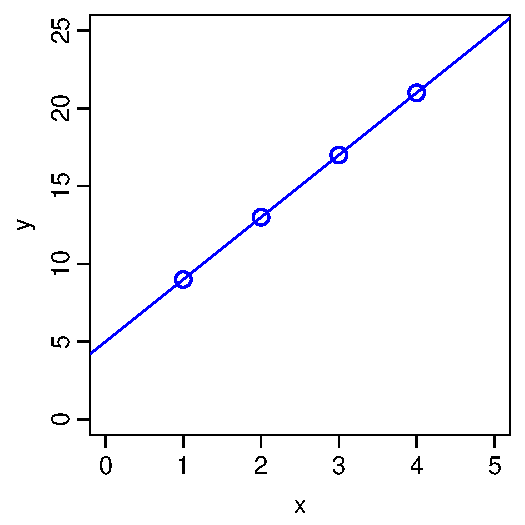
\includegraphics[width=\textwidth]{Intercept.pdf}
		
	\column{0.5\textwidth}
		\begin{align*}
		  y  &= \beta_1 + \beta_2 x \\
		  \\
		  9  &= 5 + 4 \times 1 \\
		  13  &= 5 + 4 \times 2 \\
		  21 &= 5 + 4 \times 3 \\
		  29 &= 5 + 4 \times 4   
		\end{align*}
        \[\beta_1 = 5; \beta_2=4\]
\end{columns}
}

\frame
{\frametitle{Examples - one factor}

\begin{columns}[T]

	\column{0.5\textwidth}
		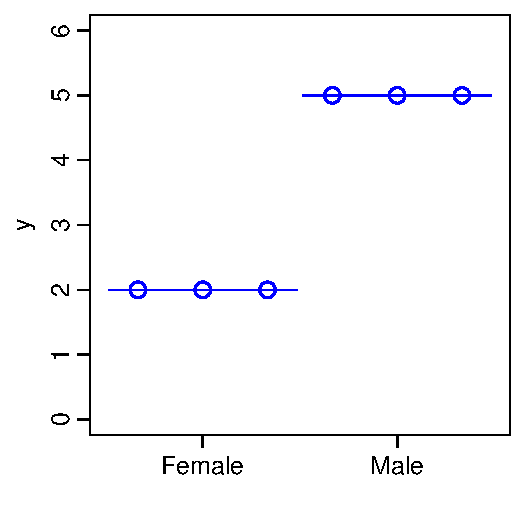
\includegraphics[width=\textwidth]{Factor.pdf}
		
	\column{0.5\textwidth}
		\begin{align*}
		  y  &= \beta_1 + \beta_2 g_m  \\
		  \\
		  2  &= 2 + 3 \times 0 \\
		  2  &= 2 + 3 \times 0 \\
		  2  &= 2 + 3 \times 0 \\
		  5  &= 2 + 3 \times 1 \\  
		  5  &= 2 + 3 \times 1 \\
		  5  &= 2 + 3 \times 1
		\end{align*}
        \[\beta_1 = 2; \beta_2=3\]
\end{columns}
}


\frame
{\frametitle{Examples - one continuous variable and one factor}

\begin{columns}[T]

	\column{0.5\textwidth}
		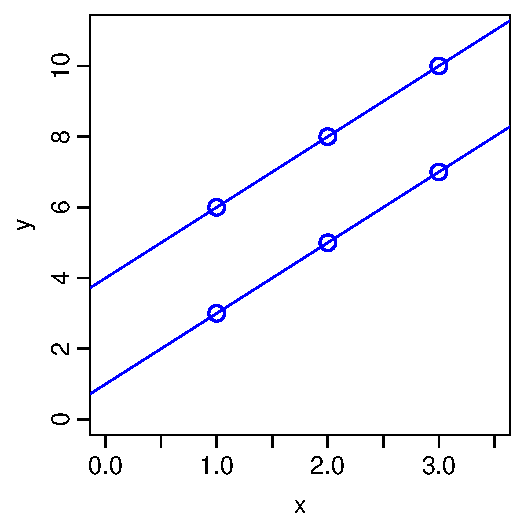
\includegraphics[width=\textwidth]{TwoVars.pdf}
		
	\column{0.5\textwidth}
		\begin{align*}
		  y  &= \beta_1  + \beta_2 x + \beta_3 g_m\\
		  \\
		  3   &= 1 + 2 \times 1 + 3 \times 0\\
		  5   &= 1 + 2 \times 2 + 3 \times 0\\
		  7   &= 1 + 2 \times 3 + 3 \times 0\\
		  6   &= 1 + 2 \times 1 + 3 \times 1\\  
		  8   &= 1 + 2 \times 2 + 3 \times 1\\
		  10  &= 1 + 2 \times 3 + 3 \times 1
		\end{align*}
        \[\beta_1 = 1; \beta_2=2; \beta_3=3\]
\end{columns}
}



\frame
{\frametitle{Examples - one continuous variable and one factor}

\begin{columns}[T]

	\column{0.5\textwidth}
		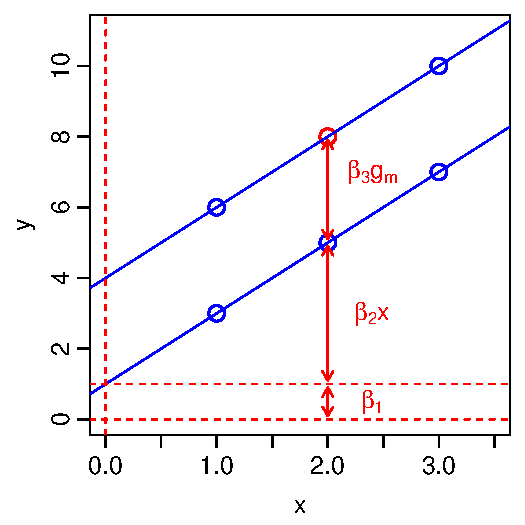
\includegraphics[width=\textwidth]{TwoVarsHighlight.pdf}
		
		\column{0.5\textwidth}
			\begin{align*}
			  y  &= \beta_1  + \beta_2 x + \beta_3 g_m\\
			  \\
			  3   & = 1 + 2 \times 1 + 3 \times 0\\
			  5   & = 1 + 2 \times 2 + 3 \times 0\\
			  7   & = 1 + 2 \times 3 + 3 \times 0\\
			  6   & = 1 + 2 \times 1 + 3 \times 1\\  
			  {\color{red}8} & {\color{red}\;= 1 + 2 \times 2 + 3 \times 1}\\ % loses a space for some reason
			  10  & = 1 + 2 \times 3 + 3 \times 1
			\end{align*}
	        \[\beta_1 = 1; \beta_2=2; \beta_3=3\]
\end{columns}
}

\section{How do we deal with variation?}


\frame
{\frametitle{Residuals - variation is everywhere}

\begin{center}
		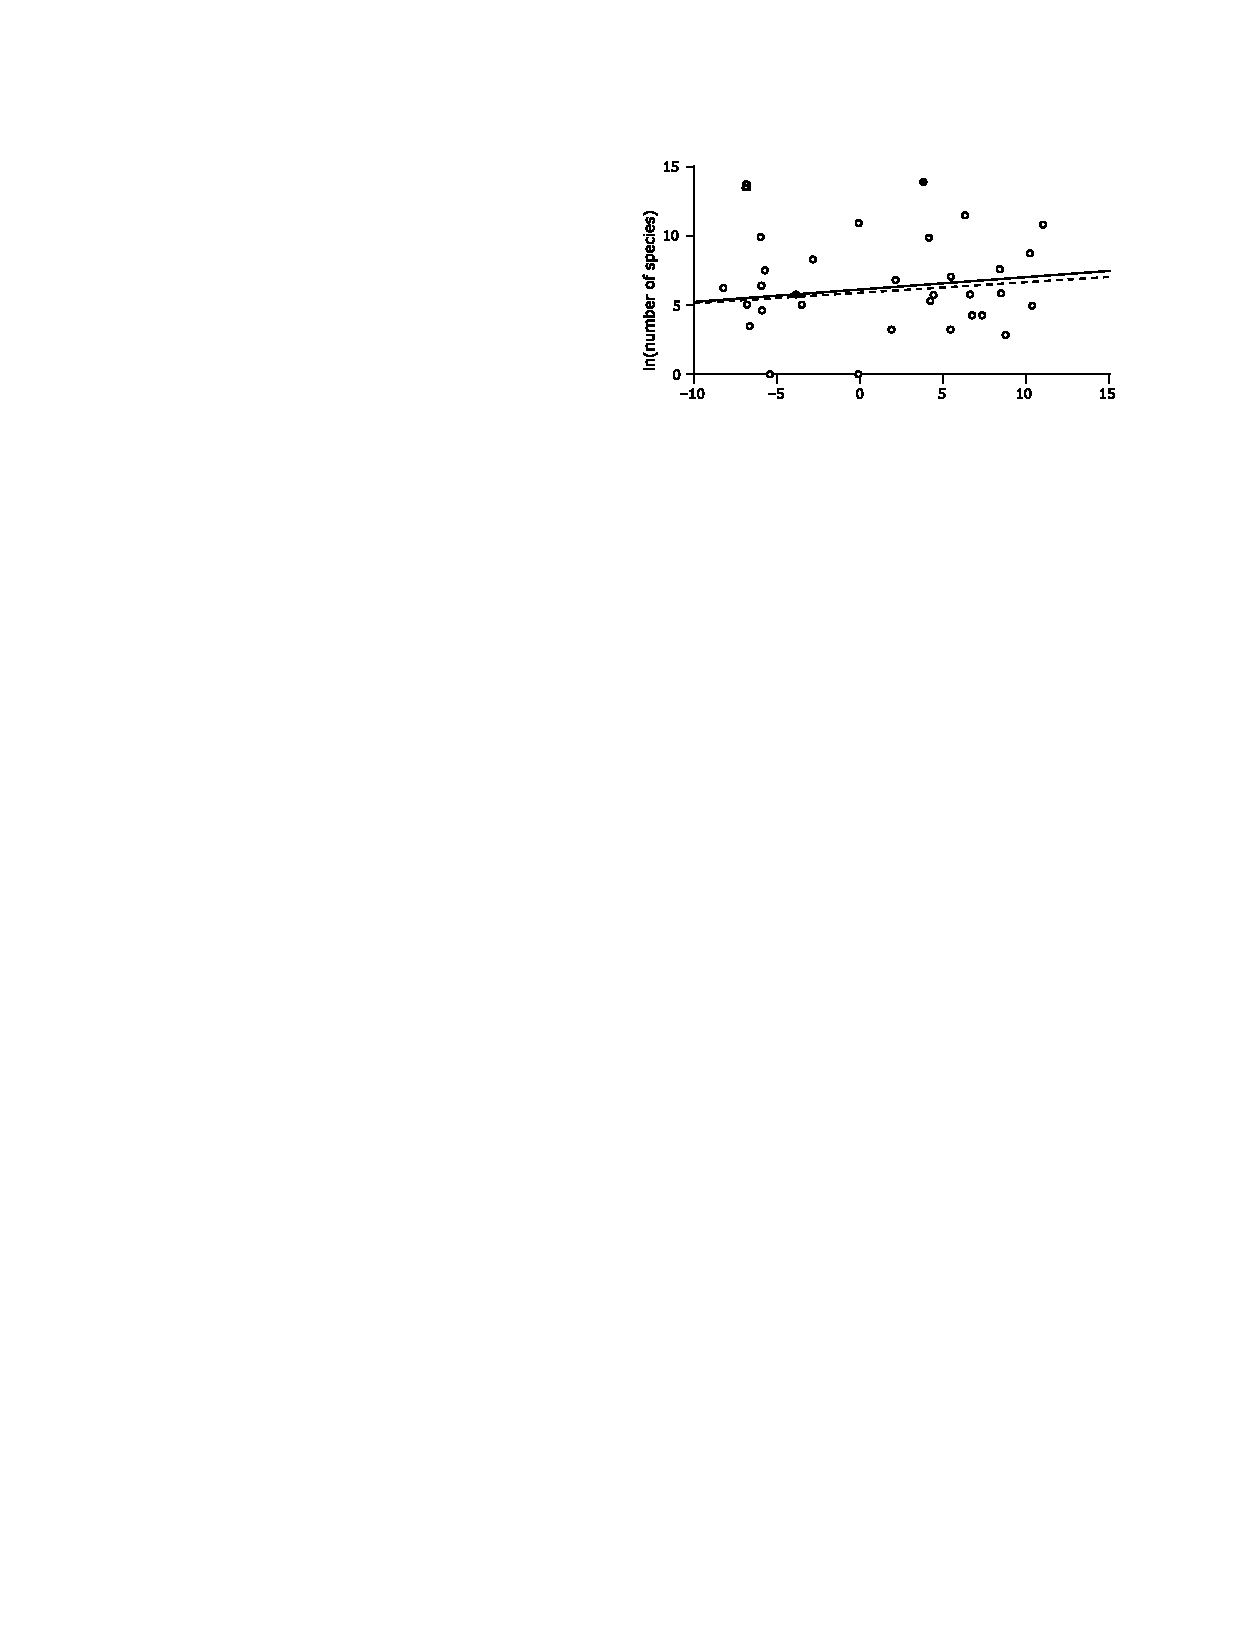
\includegraphics[width=0.6\textwidth]{VariationOrme2002.pdf}\\
		{\tiny ln(volume)}
\end{center}		
		
\begin{itemize}
\item Data always shows variation from a perfect model
\begin{itemize}
\item Missing variables (age, lab vs. field biology, time of day) 
\item Measurement error 
\item Stochastic variation
\end{itemize}
\end{itemize}
}


\frame
{\frametitle{Residuals - variation is everywhere}

\begin{columns}[T]

	\column{0.5\textwidth}
		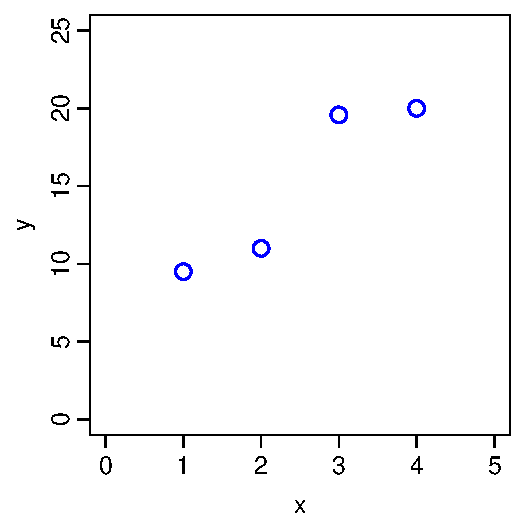
\includegraphics[width=\textwidth]{Error.pdf}
		
	\column{0.5\textwidth}
		\begin{align*}
		  y  &= \beta_1 + \beta_2 x \\
		  \\
		  9.50  &= \;?\; + \;?\; \times 1 \\
		  11.00 &= \;?\; + \;?\; \times 2 \\
		  19.58 &= \;?\; + \;?\; \times 3 \\
		  20.00 &= \;?\; + \;?\; \times 4   
		\end{align*}
		
		\begin{center}
		 {\it No unique line through the points unless we impose some other 
		 constraint or condition}
		\end{center}
		 
\end{columns}
}



\frame
{\frametitle{Residuals - Guess 1}
 \begin{columns}[T]

	\column{0.5\textwidth}
		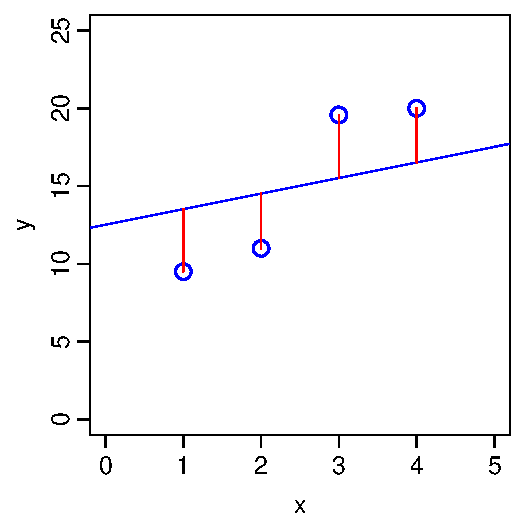
\includegraphics[width=\textwidth]{TooFlat.pdf}
		
	\column{0.5\textwidth}
		\begin{align*}
		  y  &= \beta_1 + \beta_2 x  + {\color{red} \varepsilon }\\
		  \\
		  9.50  &= 12.52 + 1 \times 1 - {\color{red} 4.02}\\
		  11.00 &= 12.52 + 1 \times 2 - {\color{red} 3.52}\\
		  19.58 &= 12.52 + 1 \times 3 + {\color{red} 4.06}\\
		  20.00 &= 12.52 + 1 \times 4 + {\color{red} 3.48} 
		\end{align*}
		\[\beta_1 = 12.52; \beta_2=1\]

\end{columns}
}


\frame
{\frametitle{Residuals  - Guess 2}
\begin{columns}[T]

	\column{0.5\textwidth}
		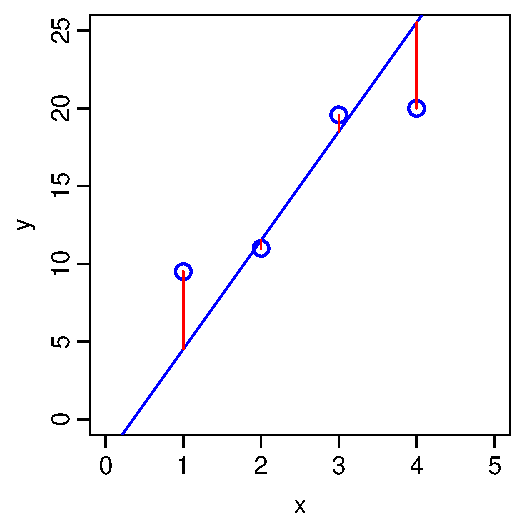
\includegraphics[width=\textwidth]{TooSteep.pdf}
		
	\column{0.5\textwidth}
		\begin{align*}
		  y  &= \beta_1 + \beta_2 x + {\color{red} \varepsilon }\\
		  \\
		  9.50  &= -2.48 + 7 \times 1 + {\color{red} 4.98}\\
		  11.00 &= -2.48 + 7 \times 2 - {\color{red} 0.52}\\
		  19.58 &= -2.48 + 7 \times 3 + {\color{red} 1.06}\\
		  20.00 &= -2.48 + 7 \times 4 - {\color{red} 5.52} 
		\end{align*}
		\[\beta_1 = -2.48; \beta_2=7\]

\end{columns}		
}


\frame
{\frametitle{Residuals - least squares solution}

Minimize the {\it sum} of the {\it squared} residuals

% %% animate directly from a multipage pdf - this is rather sweet!
% %% this is also over-engineered using timeline to only embed the axes once!
\begin{columns}[T]
\column{\textwidth}
\animategraphics[width=\textwidth, 
                 controls, %autoplay, %palindrome, 
                 timeline=Varying_timeline.txt, 
                 buttonsize=1em]{12}{Varying_timeline}{}{}

\end{columns}
}


\frame
{\frametitle{Why guess?: The least squares solution}

\begin{columns}[T]

	\column{0.5\textwidth}
		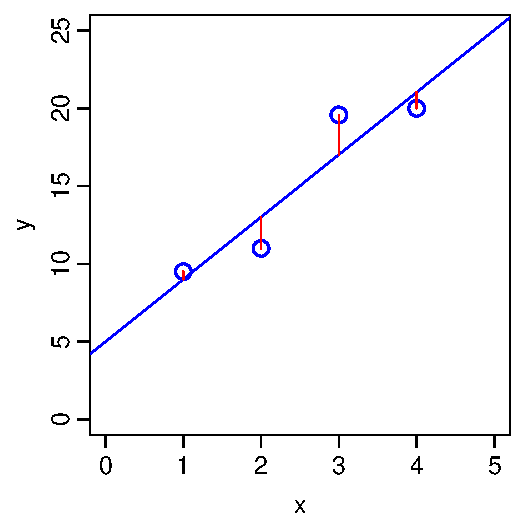
\includegraphics[width=\textwidth]{JustRight.pdf}
		
	\column{0.5\textwidth}
		\begin{align*}
		  y  &= \beta_1 + \beta_2 x  + {\color{red} \varepsilon }\\
		  \\
		  9.50  &= 5 + 4 \times 1 + {\color{red} 0.50}\\
		  11.00 &= 5 + 4 \times 2 - {\color{red} 2.00}\\
		  19.58 &= 5 + 4 \times 3 + {\color{red} 2.58}\\
		  20.00 &= 5 + 4 \times 4 - {\color{red} 1.00} 
		\end{align*}
		
		\[\beta_1 = 5; \beta_2=4\]
				
\end{columns}		
}



%	
%	\frame
%	{\frametitle{Model as a matrix - terminology}
%	
%	\begin{center}
%	
%	{\LARGE $\mathbf{Y} = \mathbf{X \beta  +  \varepsilon}$}
%	
%	\vspace{5mm}
%	
%	\begin{tikzpicture}
%	% minimum height on nodes to align labels above components
%	\begin{scope}[every node/.style={minimum height=22mm}]
%	\node                    (Y)  {$\left[ \begin{array}{c} y_1 \\ y_2 \\ y_3 \\ y_4 \end{array}\right]$};
%	\node [right= 2mm of Y]  (eq) {$=$};                                     
%	\node [right= 2mm of eq] (X)  {$\left[ \begin{array}{cc} 1 & x_1 \\ 1 & x_2 \\ 1 & x_3 \\ 1 & x_4 \end{array}\right]$};
%	\node [right= 0mm of X]  (b)  {$\left[ \begin{array}{c} \beta_1 \\ \beta_2 \end{array}\right]$};
%	\node [right= 2mm of b]  (pl) {$+$};
%	\node [right= 2mm of pl] (e)  {$\left[ \begin{array}{c} \varepsilon_1 \\ \varepsilon_2 \\ \varepsilon_3 \\ \varepsilon_4 \end{array}\right]$};
%	\end{scope}
%	
%	\begin{scope}[every node/.style={rounded corners, draw, fill=red!10},
%	              every path/.style={latex-, draw=red, thick, fill=red}]
%	
%	
%		\node [above= 5mm of Y] (obs) {Observed values};
%		\node [below= 5mm of X] (mat) {Model matrix};
%		\node [above= 5mm of b] (coe) {Coefficients};
%		\node [below= 5mm of e] (res) {Residuals};
%		\draw (Y) -- (obs);
%		\draw (X) -- (mat);
%		\draw (b) -- (coe);
%		\draw (e) -- (res);
%	
%	
%	\end{scope}
%	
%	\end{tikzpicture}
%	\end{center}
%	}



\frame
{\frametitle{Model as a matrix - terminology}

\begin{center}

{\LARGE $\mathbf{Y} = \mathbf{X \beta  +  \varepsilon}$}

\vspace{5mm}

\begin{tikzpicture}
% minimum height on nodes to align labels above components
\begin{scope}[every node/.style={minimum height=22mm}]
\node                    (Y)  {$\left[ \begin{array}{r@{}l}
 								   \alert<2>  {9} & \alert<2>{.50} \\ 
								   \alert<3> {11} & \alert<3> {.00} \\ 
                                    \alert<4> {19} & \alert<4> {.58} \\ 
                                    \alert<5> {20} & \alert<5> {.00}  \end{array}\right]$};
\node [right= 2mm of Y]  (eq) {$=$};                                     
\node [right= 2mm of eq] (X)  {$\left[ \begin{array}{cc} \alert<2>{1} & \alert<2>{1} \\
                                     \alert<3>{1} & \alert<3>{2} \\ 
                                     \alert<4>{1} & \alert<4>{3} \\ 
                                     \alert<5>{1} & \alert<5>{4} \\ \end{array}\right]$};
\node [right= 0mm of X]  (b)  {$\left[ \begin{array}{c} \alert<2-5>{5} \\ 
                                    \alert<2-5>{4} \end{array}\right]$};
\node [right= 2mm of b]  (pl) {$+$};
\node [right= 2mm of pl] (e)  {$\left[ \begin{array}{r@{}l} 
								   \alert<2>  {0} & \alert<2>{.50} \\ 
								   \alert<3> {-2} & \alert<3> {.00} \\ 
                                    \alert<4>  {2} &\alert<4> {.58} \\ 
                                    \alert<5> {-1} & \alert<5> {.00}  \end{array}\right]$};
\end{scope}

\begin{scope}[every node/.style={rounded corners, draw, fill=red!10},
              every path/.style={latex-, draw=red, thick, fill=red}]

\onslide<1-5>{
	\node [above= 5mm of Y] (obs) {Observed values};
	\node [below= 5mm of X] (mat) {Model matrix};
	\node [above= 5mm of b] (coe) {Coefficients};
	\node [below= 5mm of e] (res) {Residuals};
	\draw (Y) -- (obs);
	\draw (X) -- (mat);
	\draw (b) -- (coe);
	\draw (e) -- (res);
}

\onslide<6>{
	\node [above= 5mm of eq, minimum width=38mm] (given) {Given these \ldots};
	\node [above= 5mm of b, xshift=18mm] (find) {\ldots find the set of these\ldots};
	\node [below= 5mm of b] (min)  {\ldots that minimize the sum of the squares of these.};

	\draw (Y.north) -- (Y.north |- given.south);
	\draw (X.north) -- (X.north |- given.south);
	\draw (b.north) -- (b.north |- find.south);
	\draw (e.south) -- (e.south |- min.north);   
}

\end{scope}

\end{tikzpicture}
\end{center}
}

\frame
{\frametitle{Model as a matrix - predictions}

\begin{center}

{\LARGE $\mathbf{\hat{Y}} = \mathbf{X \beta }$}

\vspace{5mm}

\begin{tikzpicture}
% minimum height on nodes to align labels above components
\begin{scope}[every node/.style={minimum height=22mm}]
\node                    (Y)  {$\left[ \begin{array}{c} {9} \\ 
                                     {13} \\ 
                                     {17} \\ 
                                     {21} \\ \end{array}\right]$};
\node [right= 2mm of Y]  (eq) {$=$};                                     
\node [right= 2mm of eq] (X)  {$\left[ \begin{array}{cc} {1} & {1} \\
                                     {1} & {2} \\ 
                                     {1} & {3} \\ 
                                     {1} & {4} \\ \end{array}\right]$};
\node [right= 0mm of X]  (b)  {$\left[ \begin{array}{c} {5} \\ 
                                    {4} \end{array}\right]$};
\end{scope}

\begin{scope}[every node/.style={rounded corners, draw, fill=red!10},
              every path/.style={latex-, draw=red, thick, fill=red}]

	\node [above= 5mm of Y] (obs) {Predicted or fitted values};
	\node [below= 5mm of X] (mat) {Model matrix};
	\node [above= 5mm of b] (coe) {Coefficients};
	\draw (Y) -- (obs);
	\draw (X) -- (mat);
	\draw (b) -- (coe);
	
\end{scope}

\end{tikzpicture}
\end{center}
}

\frame
{\frametitle{Predicted values}

\begin{columns}[T]

	\column{0.5\textwidth}
		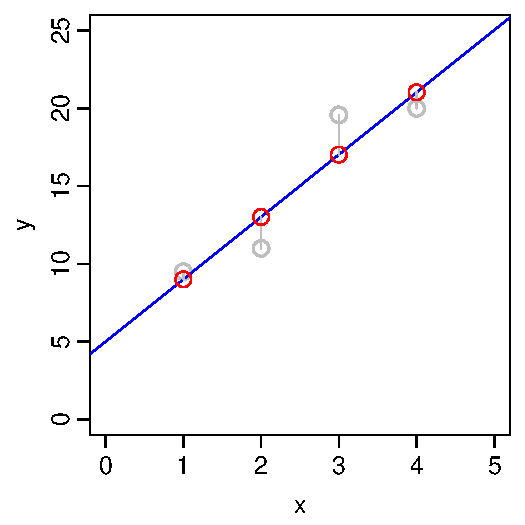
\includegraphics[width=\textwidth]{Predicted.pdf}
		
	\column{0.5\textwidth}
		\begin{align*}
		  \hat{y}  &= \beta_1 + \beta_2 x  \\
		  \\
		  9  &= 5 + 4 \times 1 \\
		  13 &= 5 + 4 \times 2 \\
		  17 &= 5 + 4 \times 3 \\
		  21 &= 5 + 4 \times 4  
		\end{align*}
\end{columns}		
}

\section{Is a linear model appropriate?}

\frame
{\frametitle{Assumptions}

\begin{itemize}\itemsep20pt
\item Linear models have the following assumptions:
\begin{itemize}
\item No measurement error in explanatory variables
\item The explanatory variables are not very highly correlated
\item \color<2>{red} The model is linear
\item \color<2>{red} The model has constant normal variance
\end{itemize}
\item {\bf If these assumptions are not met, the model can be very wrong}
\item<2> The last two need some further explanation
\end{itemize}

}

\begin{frame}[T]
\frametitle{`The model is linear'}

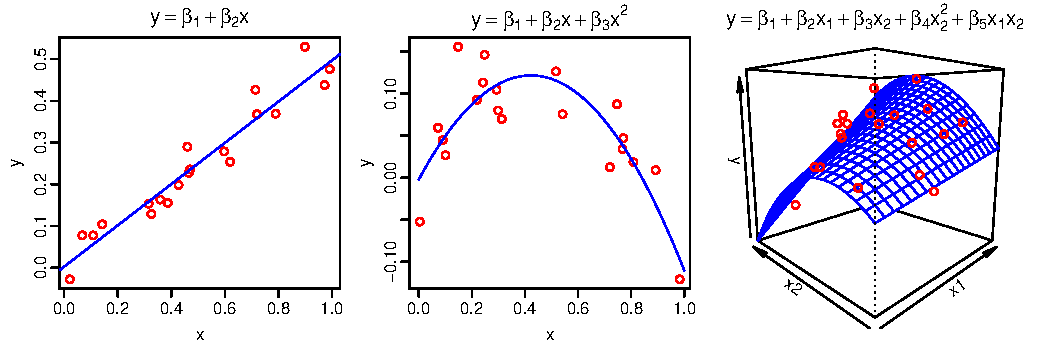
\includegraphics[width=\textwidth]{Linear.pdf}

\begin{itemize}
\item These are {\it all} good linear models.
\item Linear models can include curved relationships (e.g. polynomials)
\item The data can be modelled as a {\it sum} of components
\item A {\it linear combination} of variables and coefficients
\end{itemize}

\end{frame}



\begin{frame}[T]
\frametitle{`The model has constant normal variance'}
\begin{columns}[T]

	\column{0.5\textwidth}
		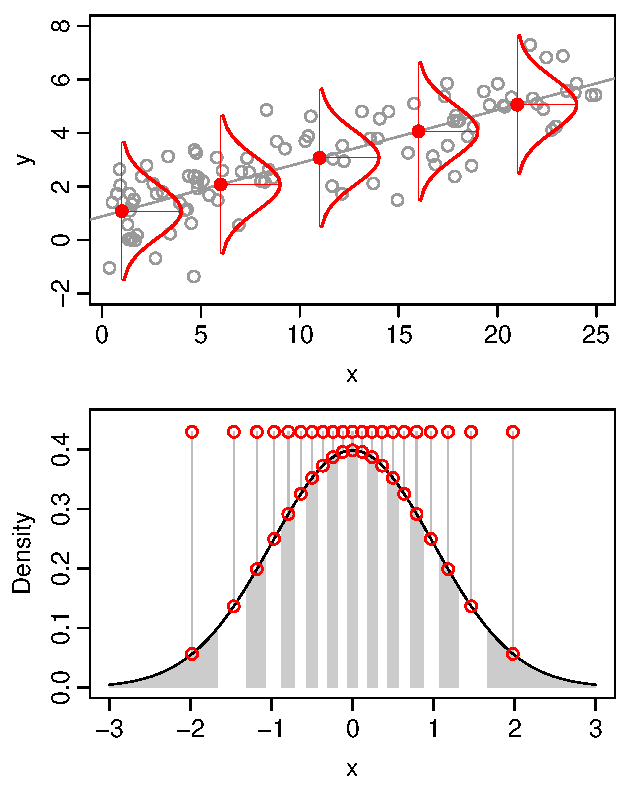
\includegraphics[height=72mm]{ResidDemo.pdf}
		
	\column{0.5\textwidth}
		\begin{itemize}
		\item The data has a similar spread around any predicted point in the model
		\vspace{2cm}
		\item The residuals are normal
		\item Points {\it should} be spaced equally in the area under the curve
		\item Expect mostly small but a few larger residuals
		\end{itemize}
		
\end{columns}
\end{frame}

\begin{frame}[T]
\frametitle{`The model has constant normal variance'}

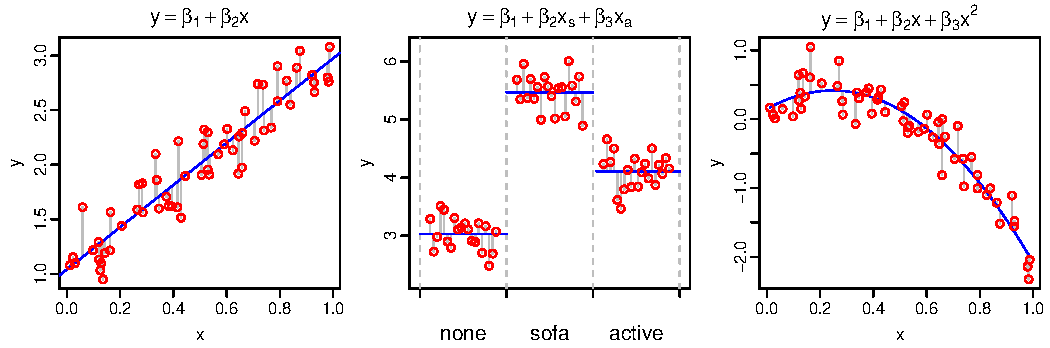
\includegraphics[width=\textwidth]{ConstantVarianceMods.pdf}

\begin{itemize}
\item Three good models
\begin{itemize}
\item Is the spread the same for all fitted values?
\item Do the residuals match the normal expectation?
\end{itemize}
\end{itemize}


\end{frame}

\begin{frame}[T]
\frametitle{`The model has constant normal variance'}

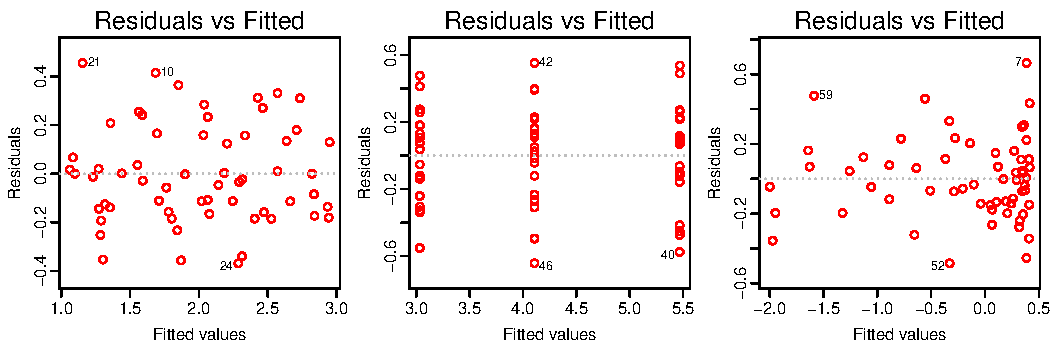
\includegraphics[width=0.95\textwidth]{FitResid.pdf}

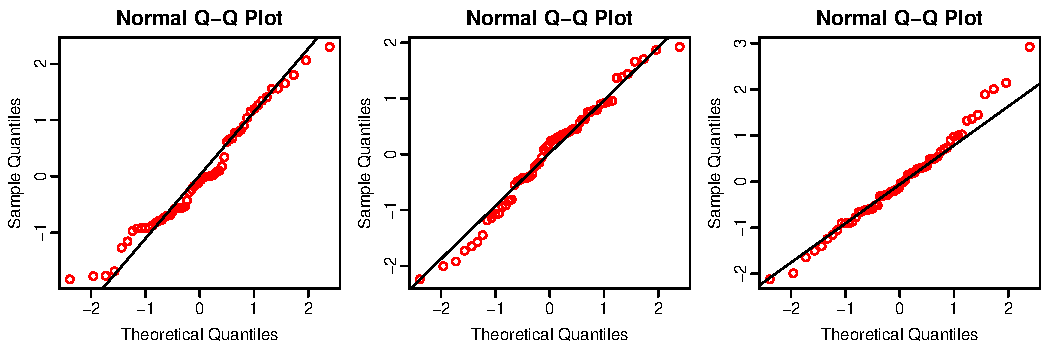
\includegraphics[width=0.95\textwidth]{QQNorm.pdf}


\end{frame}




\begin{frame}[T]
\frametitle{`The model has constant normal variance'}

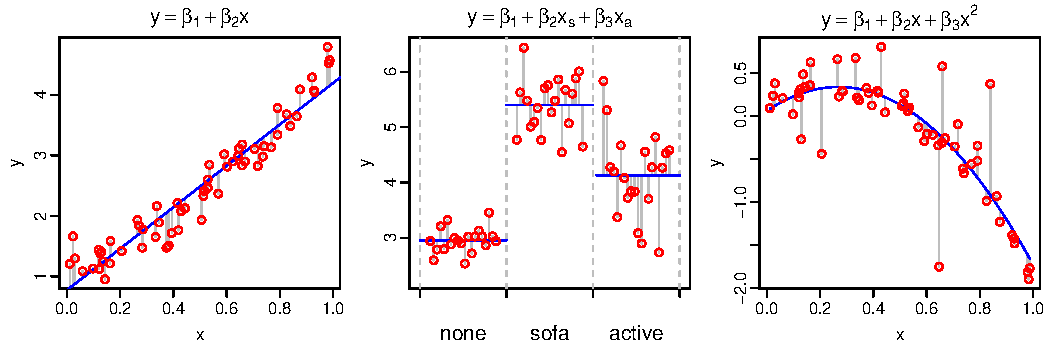
\includegraphics[width=\textwidth]{NonConstantVarianceMods.pdf}

\begin{itemize}
\item Three bad models
\begin{itemize}
\item Is the spread the same for all fitted values?
\item Do the residuals match the normal expectation?
\end{itemize}
\end{itemize}

\end{frame}

\begin{frame}[T]
\frametitle{`The model has constant normal variance'}

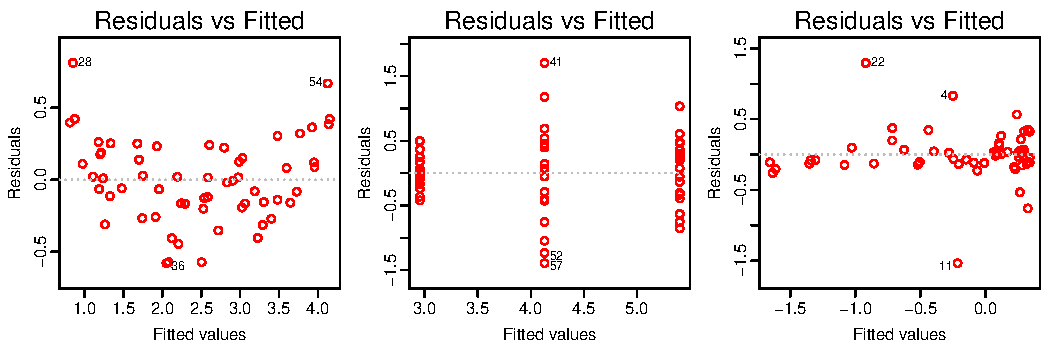
\includegraphics[width=0.95\textwidth]{BadFitResid.pdf}

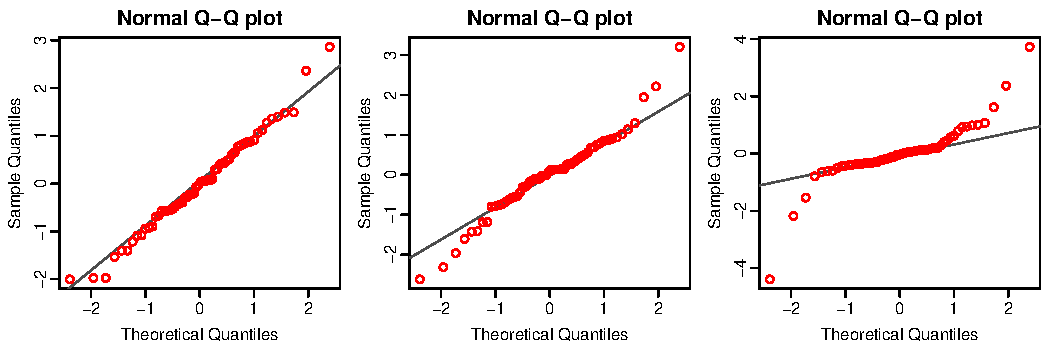
\includegraphics[width=0.95\textwidth]{BadQQNorm.pdf}

%% TODO - add labels

\end{frame}


\frame
{\frametitle{Is a linear model appropriate?}
{\centering \Huge

Plot the data!\\
Plot the residuals!

}}


\section{Is a linear model explanatory?}

\frame
{\frametitle{How explanatory is the model?}

\begin{center}
\begin{itemize}\itemsep20pt
\item Back to F and t tests! (Woohoo!)
\item {\it Terms}: analysis of variance
\begin{itemize}
\item Does the model explain enough variation?
\item Does each term explain enough variation?
\end{itemize}
\item {\it Coefficients}: $t$ tests
\begin{itemize}
\item Are the coefficients different from zero?
\end{itemize}
\end{itemize}

\end{center}
}

\begin{frame}[T]
\frametitle{Null and over-specified models - two endpoints}
\begin{columns}[T]

	\column{0.5\textwidth}
		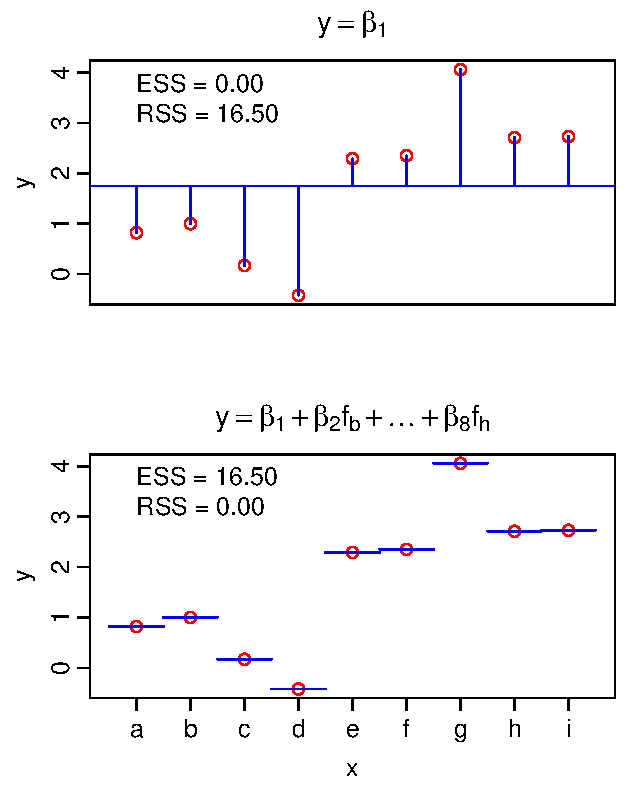
\includegraphics[height=72mm]{NullSaturated.pdf}

	\column{0.5\textwidth}
		\begin{itemize}
		\item The null model ($H_0$)
		\item Nothing is going on
		\item Biggest possible residuals
		\item Residual sum of squares (RSS) is as big as it can be
		\vspace{1cm}
		\item The saturated model
		\item One coefficient per data point
		\item RSS is zero - all the sums of squares are now explained (ESS)
		\end{itemize}
		
\end{columns}
\end{frame}


\begin{frame}[T]
\frametitle{More interesting models}


		\centerline{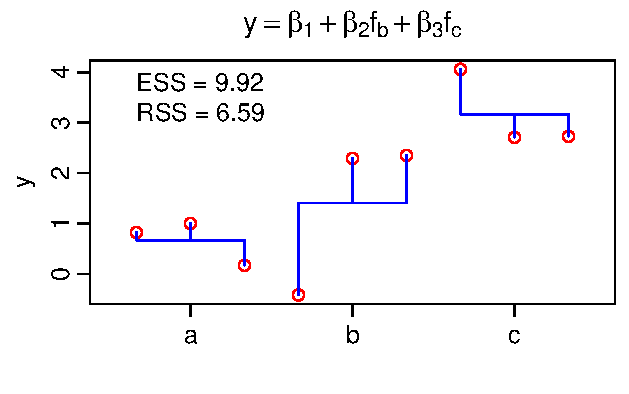
\includegraphics[height=0.5\textheight]{Intermediate.pdf}}

		\begin{itemize}
		\item Added a term with three levels
		\item Some but not all of the residual sums of squares are explained
		\item Is this enough to be interesting?
		\end{itemize}		

\end{frame}


\begin{frame}[T]
\frametitle{The F statistic}

\begin{center}

	\begin{tikzpicture}[every node/.style={ text depth=1mm, inner sep=2mm,font=\Large}, node distance=0mm]
	
	\node (stat) {F};
	\node (eq1) [right= of stat] {=};

	\matrix (ratio1) [right=of eq1,ampersand replacement=\&] {
		\node (ESS) {ESS}; \node(div1) [right=of ESS] {/}; \node (Nc) [right= of div1]{$N_c$} ; \\ 
		\node (RSS) 	{RSS}; \node(div2) [right=of RSS]{/}; \node (Nr) [right= of div2]{$N_r$} ;\\
	};

	\draw (ESS.south west) -- (Nc.south east);
	\node (eq2) [right= of ratio1] {=};

	\matrix (ratio2)[right=of eq2,ampersand replacement=\&] {
		\node (ESSn) {9.92}; \node(div3) [right=of ESSn] {/}; \node (Ncn) [right= of div3]{$2$} ; \\ 
		\node (RSSn) {6.59}; \node(div4) [right=of RSSn]{/}; \node (Nrn) [right= of div4]{$6$} ;\\
	};

	\draw (ESSn.south west) -- (Ncn.south east);
	
	\node (eq3) [right= of ratio2] {=};
	\node (res) [right= of eq3] {4.52};
	
	\begin{scope} [every node/.style={fill=blue!10, draw=blue, font=\large, rounded corners, align=center},
                   every path/.style={latex-,  thick, draw=blue}]
	\node (ESSGood)  [above=of ESS, yshift=8mm, xshift=-4mm] {Large ESS \\ is good};	
	\node (RSSGood)  [below=of RSS, yshift=-8mm, xshift=-4mm] {Small RSS \\ is good};	
	\node (NcGood)  [above=of Nc, yshift=8mm, xshift=8mm, anchor=south west] {Fewer coefficients \\ is better};	
	\node (NrGood)  [below=of Nr, yshift=-8mm, xshift=8mm, anchor=north west] {Residual degrees of freedom};	
	
	\draw [blue] (ESS.north) -- (ESS.north |- ESSGood.south);
	\draw  [blue](RSS.south) -- (RSS.south |- RSSGood.north);
	\draw [blue] (Nc.north) |- (NcGood.west);
	\draw [blue] (Nr.south) |- (NrGood.west);

	
	\end{scope}
	
	\end{tikzpicture}

\end{center}

\end{frame}


\begin{frame}[T]
\frametitle{$F$ values by chance}

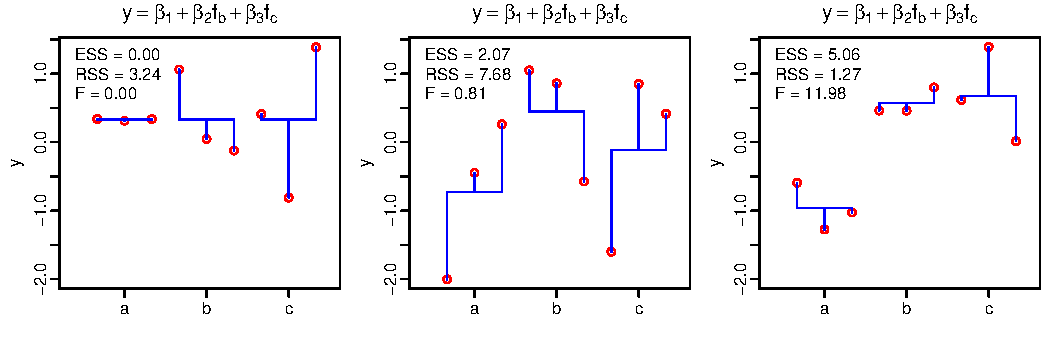
\includegraphics[width=\textwidth]{F_extremes.pdf}

\begin{itemize}
\item What is the distribution of $F$ if nothing is going on?
\item Simulate 10,000 datasets where nothing is going on ($H_0$ is true)
\item Calculate $F$ for each random dataset under $H_1$
\item Mostly $H_1$ has a low $F$ - but sometimes it is high by chance 
\end{itemize}

\end{frame}


% 

\begin{frame}[T]
\frametitle{Distribution of $F$}

% %% animate directly from a multipage pdf - this is rather sweet!
% %% this is also over-engineered using timeline to only embed the axes once!

\centerline{\animategraphics[height=0.5\textheight, 
                 %autoplay, %controls, %palindrome, 
                 timeline=FAnimate.txt, 
                 buttonsize=1em]{12}{FAnimate}{}{}}

\begin{itemize}
\item In our possibly interesting model, $F=4.52$
\item<2> 95\% of the random data sets have $F\le 5.5$
\item<2> A model this good is found by chance 1 in 16 times ($p=0.063$)
\item<2> Not quite interesting enough!
\end{itemize}

\end{frame}


\begin{frame}[T]
\frametitle{Are coefficients different from zero?}


\begin{center}

	\begin{tikzpicture}[every node/.style={ text depth=1mm, inner sep=2mm,font=\Large}, node distance=0mm]
	
	\node (stat) {t};
	\node (eq1) [right= of stat] {=};

	\matrix (ratio1) [right=of eq1,ampersand replacement=\&] {
		\node (diff) {Effect size}; \\ 
		\node (prec) 	{Precision}; \\
	};
	\draw (diff.south west) -- (diff.south east);
	
	\node (eq2) [right= of ratio1] {=};

	\matrix (ratio2) [right=of eq2,ampersand replacement=\&] {
		\node (val) {Coefficient value}; \\ 
		\node (se) 	{Standard error}; \\
	};
	\draw (val.south west) -- (val.south east);
	
	\begin{scope} [every node/.style={fill=blue!10, draw=blue, font=\large, rounded corners, align=center},
                   every path/.style={latex-,  thick, draw=blue}]
	\node (esgood)  [above=of eq2, yshift=10mm ] {Large is good - bigger changes};	
	\node (precgood)  [below=of eq2, yshift=-10mm] {Small is good - known more precisely};	
	
	\draw [blue] (diff.north) -- (diff.north |- esgood.south);
	\draw [blue] (val.north) -- (val.north |- esgood.south);
	\draw [blue] (prec.south) -- (prec.south |- precgood.north);
	\draw [blue] (se.south) -- (se.south |- precgood.north);	
		
	\end{scope}
	
	\end{tikzpicture}
\end{center}


\begin{itemize}
\item The value of a coefficient in a model is an {\it effect size}
\item How much does changing this variable change the response?
\item A {\it standard error} estimates how precisely we know the value
\end{itemize}


\end{frame}

\begin{frame}[T]
\frametitle{Variation in effect size and precision}


	
		\centerline{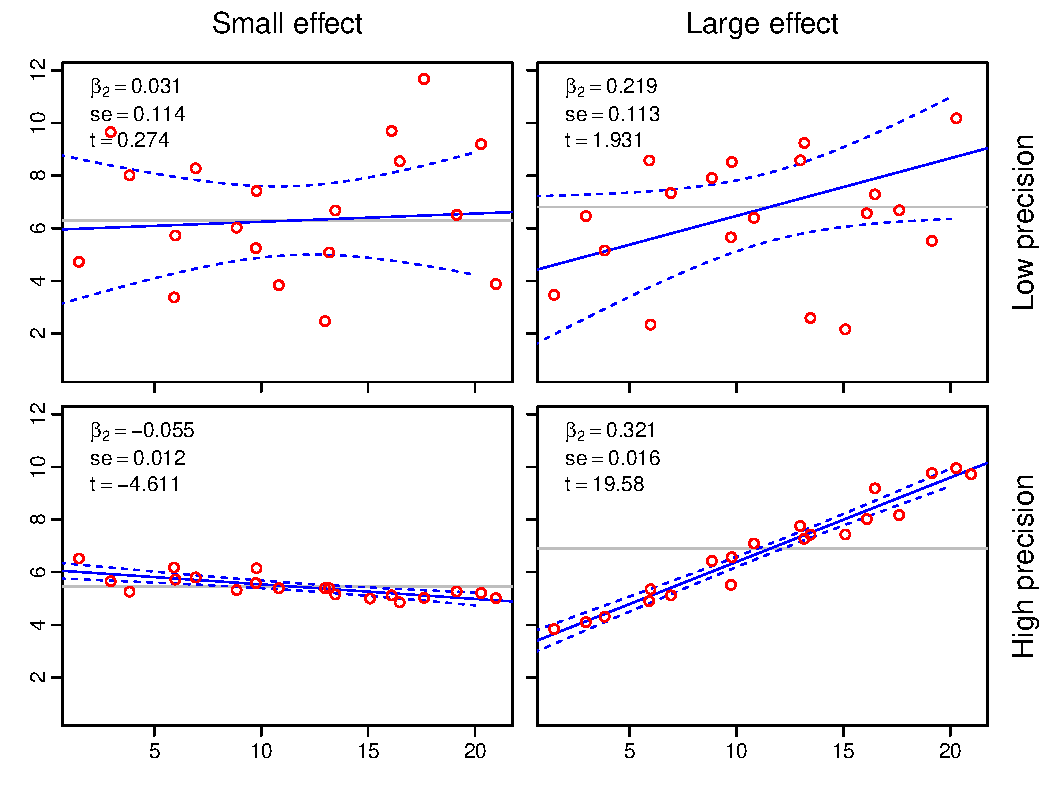
\includegraphics[height=75mm]{T_examples.pdf}}


\end{frame}


\begin{frame}[T]
\frametitle{$t$ values by chance}

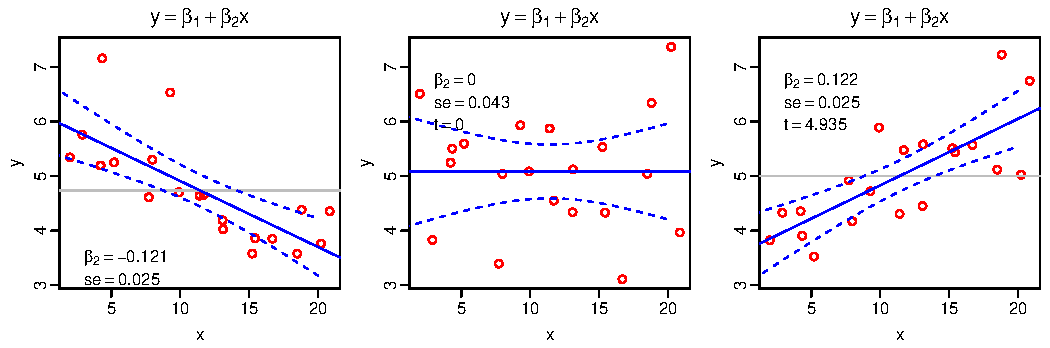
\includegraphics[width=\textwidth]{t_extremes.pdf}

\begin{itemize}
\item What is the distribution of $t$ if nothing is going on?
\item Simulate 10,000 datasets where nothing is going on ($H_0$ is true)
\item Calculate $t$ for each random dataset under $H_1$
\item Mostly $H_1$ has a $t$ near zero but can be positive or negative
\end{itemize}

\end{frame}

% 

\begin{frame}[T]
\frametitle{Distribution of $t$}

% %% animate directly from a multipage pdf - this is rather sweet!
% %% this is also over-engineered using timeline to only embed the axes once!

\centerline{\animategraphics[height=0.5\textheight, 
                 %autoplay, %controls, %palindrome, 
                 timeline=FAnimate.txt, 
                 buttonsize=1em]{12}{tAnimate}{}{}}

\begin{itemize}
\item 95\% of the random data sets have $t\le \pm 2.09$
\item Only the two higher precision models are expected to occur less than 1 time in 20 by chance.
\end{itemize}

\end{frame}

\begin{frame}[T]
\frametitle{Summary}

\begin{itemize}
\item Linear models predict a continuous response variable
\item A sum based on the effect size of explanatory variables
\item Estimate the model using least squares residuals
\item Need to check if the model is appropriate
\item Then check if the model is explanatory
\end{itemize}

\end{frame}



\begin{frame}[T]
\frametitle{What about Analysis of Variance (ANOVA)?}

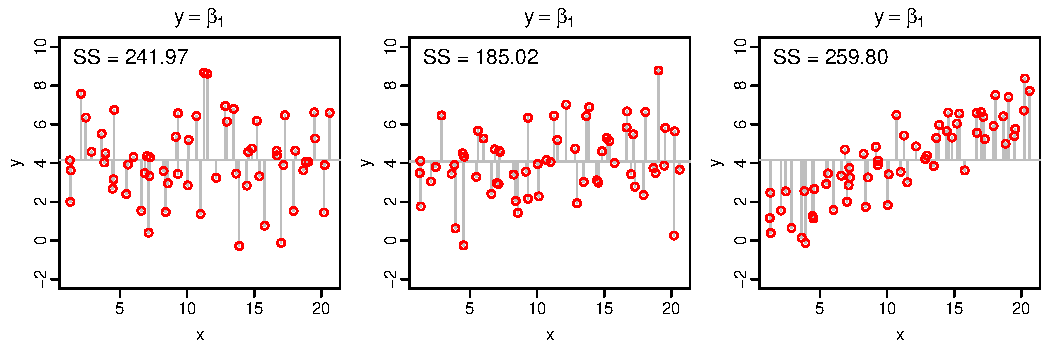
\includegraphics[width=\textwidth]{ANOVA_null.pdf}

\begin{itemize}
\item The null hypothesis ($H_0$): Nothing is going on
\item The residuals have to get smaller as we include terms.
\item How much shorter?
\end{itemize}

\end{frame}



\begin{frame}[T]
\frametitle{Examples: one continuous term}

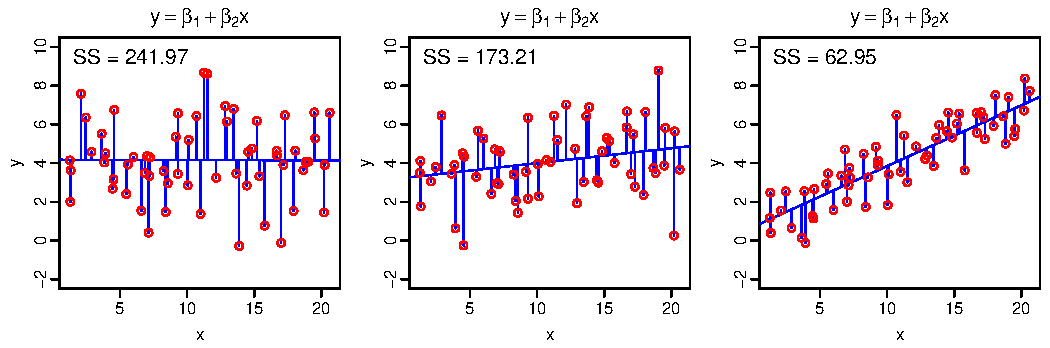
\includegraphics[width=\textwidth]{ANOVA_mod.pdf}

\begin{itemize}
\item An alternative model ($H_1$) using $x$
\item Added one term ($x$) to the model to give ($H_1$)
\item Do we reject $H_0$ and accept this new model?
\end{itemize}

\end{frame}


\begin{frame}[T]
\frametitle{Examples: adding a factor}

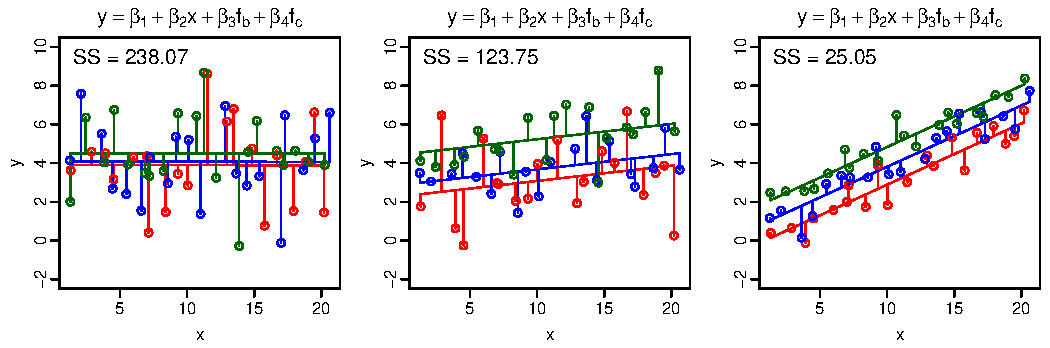
\includegraphics[width=\textwidth]{ANOVA_mod2.pdf}

\begin{itemize}
\item Another model ($H_2$) using $x$ and a factor $f$ with three levels
\item The sum of squares gets smaller again 
\item We've added one term ($f$) but two coefficients ($f_b$ and $f_c$)
\item Is this even better than $H_1$?
\end{itemize}

\end{frame}


\begin{frame}[T]
\frametitle{Change in variance}

\begin{table}[htdp]
	\begin{center}
		\begin{tabular}{ccccc}
				&  & Model A & Model B & Model C \\
		\hline
		$H_0 $ & Unexplained SS & 241.97 & 185.02 & 259.80 \\
		       & Explained SS   & 0      & 0      &    0   \\
		$H_1 $ & Unexplained SS & 241.97 & 173.21 & 62.95 \\
		       & Explained SS   & 0.00  & 11.81 & 196.85 \\
		$H_2 $ & Unexplained SS & 238.07 & 123.75 & 25.05 \\
		       & Explained SS   & 3.9  & 61.27 & 234.75 \\
		\end{tabular}
	\end{center}
\end{table}

\end{frame}


	% 
	% \frame
	% {\frametitle{How to find $\beta$ \dots}
	% 
	% \begin{center}
	% \begin{tikzpicture}
	% 
	% \node                     (eq1)  {=};
	% \node [left=  2mm of eq1] (lhs1) {$\mathbf{Y}$};
	% \node [right= 2mm of eq1] (rhs1) {$\mathbf{X \beta  +  \varepsilon}$};
	% \node [below= 7mm of eq1] (eq2)  {=};
	% \node [left=  2mm of eq2] (lhs2) {$\mathbf{X^T Y}$};
	% \node [right= 2mm of eq2] (rhs2) {$\mathbf{X^T X \beta}$};
	% \node [below= 7mm of eq2] (eq3)  {=};
	% \node [left=  2mm of eq3] (lhs3) {$\mathbf{(X^T X )^{-1} X^T Y}$};
	% \node [right= 2mm of eq3] (rhs3) {$\mathbf{\beta}$};
	% 
	% 
	% \end{tikzpicture}
	% \end{center}
	% 
	% }
	% 
	% 
% 
% \frame
% {\frametitle{Categorical variables}
% \begin{columns}[T]
% 
% \column{0.5\textwidth}
	% 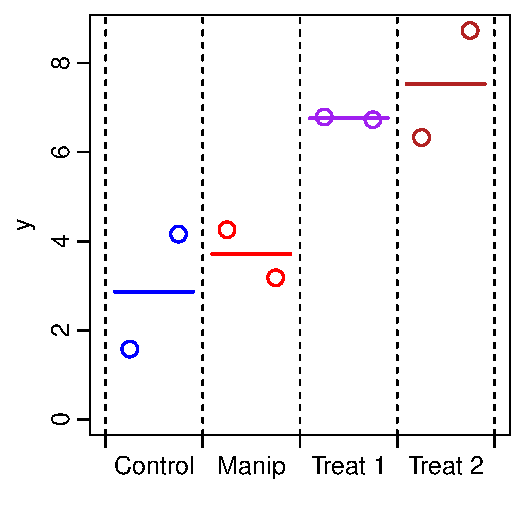
\includegraphics[width=\textwidth]{Anova.pdf}
	% 
% \column{0.5\textwidth}
	% Features of categorical variables\\
	% \begin{itemize}
		% \item Also called {\it factors}
		% \item Have a set of discrete {\it levels}
		% \item We want to model {\it differences} between levels
		% \item The least squares estimate for a level is simply the {\it mean} within the level
		% \item How do we include this in the linear model?
	% \end{itemize}
% \end{columns}		
% }
% 

% \frame
% {\frametitle{Contrasts}
% 
% \begin{itemize}
% \item Many possible differences between levels ({\it contrasts})
% \item For 4 levels, the possible contrasts between:
% \begin{itemize}
% \item two levels
% \item a pair of levels and a third level
% \item two pairs of levels
% \item one level and the remaining three levels
% \end{itemize}
% \item Each {\it contrast} represents a possible hypothesis.
% \end{itemize}
% \vspace{3mm}
% 
	% \begin{tikzpicture}
	% 
	% \newcommand{\bb}{\node [circle,  fill=blue, inner sep=0.5mm]{} ;}
	% \newcommand{\rr}{\node [circle,  fill=red, inner sep=0.5mm]{} ;}
	% 
	% \matrix (contrasts) [matrix of nodes, ampersand replacement=\&,  BEAMER hijacks straight &
	                     % row sep=1mm, column sep=2.5mm, 
	                     % nodes={circle, fill=black!35, inner sep=0.5mm}, nodes in empty cells]
	% {
		    % \&     \& \bb \&     \& \rr \& \rr \& [4mm]  {a}{b}
		    % \& \rr \&     \& \rr \& \bb \& \bb \&     \& \rr \& \bb \& \bb \& [4mm]  {ab}{c}
	    % \rr \& \rr \&  \bb \& [4mm]  {ab}{cd}
	    % \rr \& \bb \& \bb \& \bb \\[1.5mm]  {abc}{d}
		    % \& \bb \&     \& \rr \&     \& \bb \& 
		% \rr \&     \& \bb \& \bb \&     \& \rr \& \bb \& \bb \& \bb \& \bb \& 
		% \rr \& \bb \& \rr \& 
		% \bb \& \rr \& \bb \& \bb \\[12mm]
		% \bb \&     \&     \& \bb \& \bb \&     \& 
		% \bb \& \bb \& \rr \&     \& \rr \&     \& \bb \& \bb \&     \& \rr \& 
		% \bb \& \rr \& \rr \& 
		% \bb \& \bb \& \rr \& \bb \\[1.5mm]
		% \rr \& \rr \& \rr \&     \&     \&     \&
	    % \bb \& \bb \& \bb \& \bb \& \bb \& \bb \& \rr \&     \& \rr \&     \& 
	    % \bb \& \bb \&  \bb \&
	    % \bb \& \bb \& \bb \& \rr \\
	% };
	% 
	%% Draw in background bars to clarify contrast sets
	% \begin{scope}[on background layer, every node/.style=
	                  % {rounded corners, inner sep=0.7mm,
	                    % fill=black!20}]
	                   % 
		 % \def\x{contrasts-1-\i}
		 % \def\y{contrasts-4-\i}
		 % \def\r{col-\i}		  
	     % \foreach \i in {1, 2, ..., 23} \node (\r) [fit=(\x) (\y)]{};
	% \end{scope}
	% 
	% \node[left=4mm of contrasts-1-1]{Treat 2};
	% \node[left=4mm of contrasts-2-1]{Treat 1};
	% \node[left=4mm of contrasts-3-1]{Manip};
     	% \node[left=4mm of contrasts-4-1]{Control};
	% 
			% \draw ([yshift=5mm] col-1.north west)   -- node[above, font=\footnotesize] {\{a\} v. \{b\}}   ([yshift=5mm] col-6.north east);
			% \draw ([yshift=-5mm] col-7.south west)  -- node[below, font=\footnotesize] {\{a,b\} v. \{c\}}   ([yshift=-5mm] col-16.south east);
			% \draw ([yshift=5mm] col-17.north west)  -- node[above, font=\footnotesize] {\{a,b\} v. \{c,d\}}   ([yshift=5mm] col-19.north east);
			% \draw ([yshift=-5mm] col-20.south west) -- node[below, font=\footnotesize] {\{a,b,c\} v. \{d\}}   ([yshift=-5mm] col-23.south east);
	% 
	% \end{tikzpicture}
% }	

%
%
%
%\frame
%{\frametitle{Model as a matrix - terminology}
%
%\begin{center}
%
%{\LARGE $\mathbf{Y} = \mathbf{X \beta  +  \varepsilon}$}
%
%\vspace{5mm}
%
%\begin{tikzpicture}
%% minimum height on nodes to align labels above components
%\begin{scope}[every node/.style={minimum height=22mm}]
%\node                    (Y)  {$\left[ \begin{array}{c} 
%									1.58 \\ 6.79 \\
%									4.16 \\ 6.73 \\
%									4.26 \\ 6.33 \\
%									3.18 \\ 8.73
%                                 \end{array}\right]$};
%\node [right= 2mm of Y]  (eq) {$=$};                                     
%\node [right= 2mm of eq] (X)  {$\left[ \begin{array}{cccc} 
%									1 & 0 & 0 & 0 \\  1 & 0 & 0 & 0 \\  
%									1 & 1 & 0 & 0 \\  1 & 1 & 0 & 0 \\  
%									1 & 0 & 1 & 0 \\  1 & 0 & 1 & 0 \\  
%									1 & 0 & 0 & 1 \\  1 & 0 & 0 & 1 \\ 
%                                \end{array}\right]$};
%\node [right= 0mm of X]  (b)  {$\left[ \begin{array}{c} 
%                                         \beta_1 \\ \beta_2 \\
%                                         \beta_3 \\ \beta_4 \\
%                                 \end{array}\right]$};
%                                 
%\node [right= 2mm of b]  (pl) {$+$};
%\node [right= 2mm of pl] (e)  {$\left[ \begin{array}{c} 
%                                         \varepsilon_1 \\ \varepsilon_2 \\
%                                         \varepsilon_3 \\ \varepsilon_4 \\
%                                         \varepsilon_5 \\ \varepsilon_6 \\
%                                         \varepsilon_7 \\ \varepsilon_8 \\
%                                 \end{array}\right]$};
%\end{scope}
%
%\end{tikzpicture}
%\end{center}
%}
%
%
%\frame
%{\frametitle{Categorical variables}
%\begin{columns}[T]
%
%\column{0.5\textwidth}
%	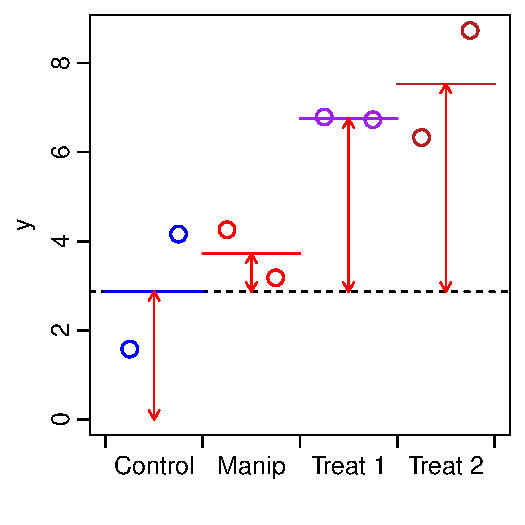
\includegraphics[width=\textwidth]{AnovaCoef.pdf}
%	
%\column{0.5\textwidth}
%\end{columns}		
%}
%
%
%
%
%\frame
%{\frametitle{Model as a matrix - terminology}
%
%\begin{center}
%
%{\LARGE $\mathbf{Y} = \mathbf{X \beta  +  \varepsilon}$}
%
%\vspace{5mm}
%
%\begin{tikzpicture}
%% minimum height on nodes to align labels above components
%\begin{scope}[every node/.style={minimum height=22mm}]
%\node                    (Y)  {$\left[ \begin{array}{c} 
%									1.58 \\ 6.79 \\
%									4.16 \\ 6.73 \\
%									4.26 \\ 6.33 \\
%									3.18 \\ 8.73
%                                 \end{array}\right]$};
%\node [right= 2mm of Y]  (eq) {$=$};                                     
%\node [right= 2mm of eq] (X)  {$\left[ \begin{array}{cccc} 
%									1 &  0.5 & -0.5 &    0 \\  1 &  0.5 & -0.5 &    0 \\  
%									1 &  0.5 &  0.5 &    0 \\  1 &  0.5 &  0.5 &    0 \\  
%									1 & -0.5 &    0 & -0.5 \\  1 & -0.5 &    0 & -0.5 \\  
%									1 & -0.5 &    0 &  0.5 \\  1 & -0.5 &    0 &  0.5 \\ 
%                                \end{array}\right]$};
%\node [right= 0mm of X]  (b)  {$\left[ \begin{array}{c} 
%                                         \beta_1 \\ \beta_2 \\
%                                         \beta_3 \\ \beta_4 \\
%                                 \end{array}\right]$};
%                                 
%\node [right= 2mm of b]  (pl) {$+$};
%\node [right= 2mm of pl] (e)  {$\left[ \begin{array}{c} 
%                                         \varepsilon_1 \\ \varepsilon_2 \\
%                                         \varepsilon_3 \\ \varepsilon_4 \\
%                                         \varepsilon_5 \\ \varepsilon_6 \\
%                                         \varepsilon_7 \\ \varepsilon_8 \\
%                                 \end{array}\right]$};
%\end{scope}
%
%\end{tikzpicture}
%\end{center}
%}
%
%
%
%\frame
%{\frametitle{Concepts}
%\begin{centering}
%  
%
%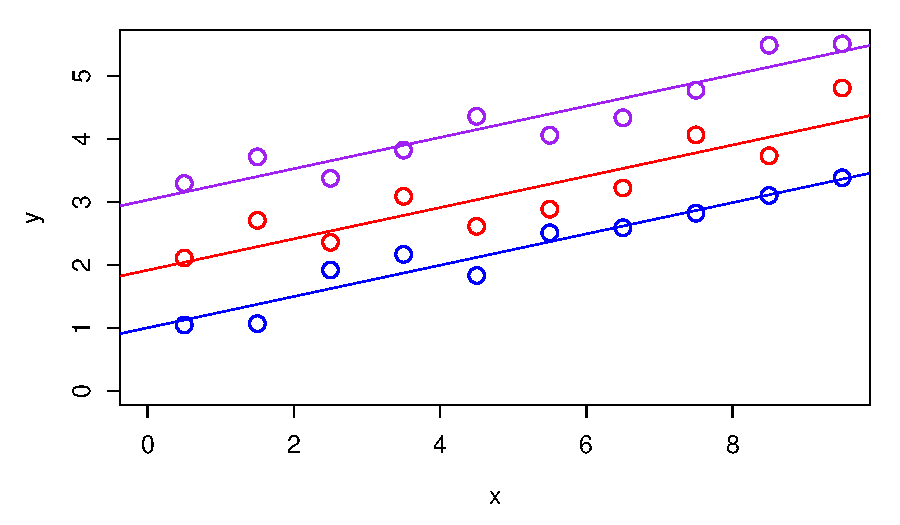
\includegraphics[width=\textwidth]{ScatterplotGroup.pdf}
%
%\end{centering}
%}
%
%\frame
%{\frametitle{Concepts}
%
%\begin{centering}
%
%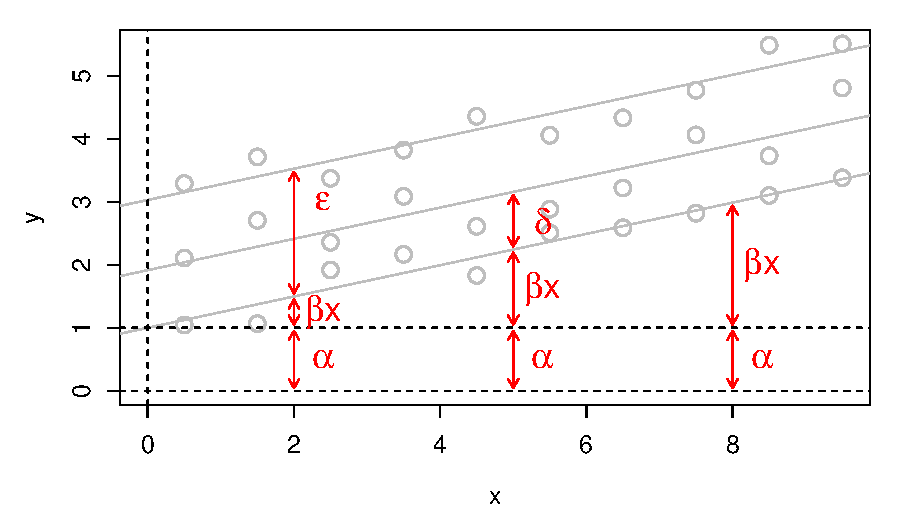
\includegraphics[width=\textwidth]{CoefMarkup.pdf}
%
%\end{centering}
%
%}
%\section{Is a linear model appropriate?}
%\frame
%{\frametitle{Concepts}
%
%\begin{centering}
%
%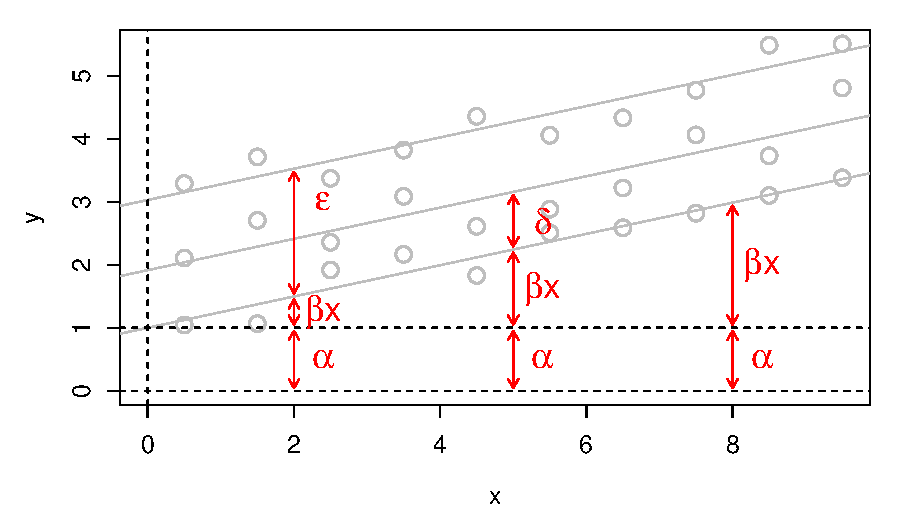
\includegraphics[width=\textwidth]{CoefMarkup.pdf}
%
%\end{centering}
%
%}
%
%\frame
%{\frametitle{Concepts}
%
%\begin{centering}
%
%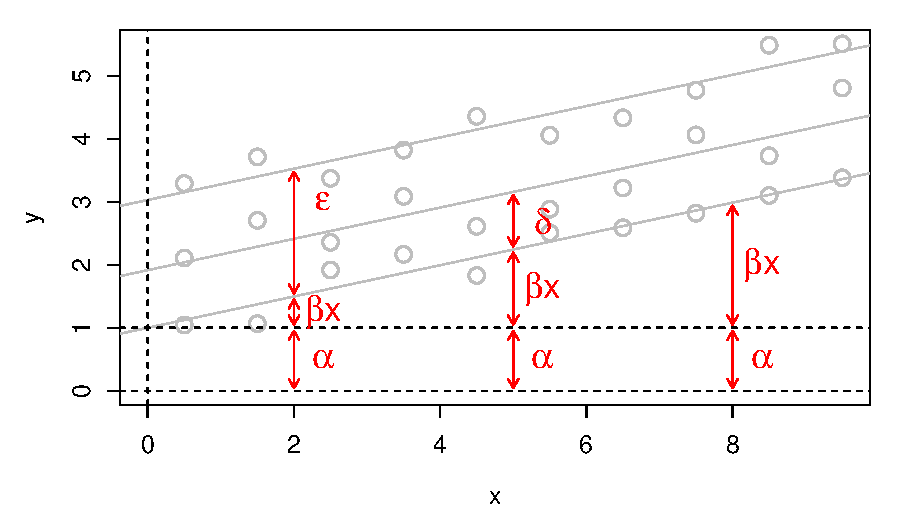
\includegraphics[width=\textwidth]{CoefMarkup.pdf}
%
%\end{centering}
%
%}

\end{document}
